%% Theorie.tex
%%
%\usepackage[ngerman]{babel}
%% ==============
\chapter{Theoretische Grundlagen}
\label{ch:Theorie}
%% ==============

{\bibliographystyle{babalpha-fl}}	% german style

Das Standardmodell der Teilchenphysik beschreibt die bisher bekannten Bausteine der Materie, sowie deren Wechselwirkungen. In Kapitel \ref{ch:Theorie:sec:Standardmodell} wird ein kurzer \"Uberblickblick dar\"uber gegeben, woraufhin in Abschnitt \cite{ch:Theorie:sec:ttH} genauer auf die Produktion von Higgs-Boson und Topquark eingegangen wird.\\


%% ===========================
\section{Das Standardmodell der Teilchenphysik}
\label{ch:Theorie:sec:Standardmodell}
%% ===========================

Der folgende Abschnitt soll einen kurzen \"Uberblick \"uber das Standardmodell der Elementarteilchenphysik geben, dabei bezieht er sich meist auf \cite{SWB-39819646X}.

Das Standardmodell der Elementarteilchenphysik ist eine Quantenfeldtheorie, die die Theorie der elektroschwachen Wechselwirkung mit der Quantenchromodynamik zusammenfasst und vereinheitlicht. Das Universum besteht aus einigen grundlegenden Bausteinen, die durch vier elementare Kr\"afte beeinflusst werden \cite{O'Luanaigh:1997201}. Die bislang beste Beschreibung dieses Aufbaus liefert das Standardmodell, wenngleich es die vierte Kraft, die Gravitation, nicht erkl/"aren kann. Dennoch war es mit diesem Modell m\"oglich fast alle experimentellen Ergebnisse zu best\"atigen, sowie sehr pr\"azise Vorhersagen \"uber verschiedene Ph\"anomene zu treffen.

Die bislang entdeckte Materie besteht aus zwei Arten von Elementarteilchen, den Leptonen sowie den Quarks. Diese lassen sich jeweils in drei Familien unterteilen. Jede Quark-Familie besteht jeweils aus einem Quarkpaar und deren Antiteilchen, diese sind Up- und Down-, Strange- und Charm-, sowie Bottom- und Topquark.\\
Leptonen bilden jeweils zusammen mit dem dazugeh\"origen Neutrino und den jeweiligen Antiteilchen eine Familie. Im Gegensatz zu den Quarks unterliegen Leptonen nicht der starken Wechselwirkung.\\
Die dritte elementare Wechselwirkung, die im Standardmodell beschrieben ist, ist die elektromagnetische Wechselwirkung. Ihr unterliegen alle geladenen Teilchen. Diese Wechselwirkungen sind in ihrer Struktur sehr \"ahnlich und werden durch den Austausch von Vektorbosonen vermittelt. Diese sind die Gluonen der starken Wechselwirkung, die W- und Z-Bosonen der schwachen Wechselwirkung und die Photonen ($\gamma$) der elektromagnetischen. W\"ahrend die Fermionen aus denen die Materie besteht, einen halbzahligen Spin besitzen, haben die Bosonen einen ganzzahligen Spin.

Der letzte fehlende Baustein im Standardmodell ist ein elementares Spin-0 Teilchen, ohne das keine konsistente Erkl\"arung f\"ur die W und Z$^0$ Massen m\"oglich w\"are. Dieses ist das Higgs-Boson, welches 2012 am CERN entdeckt wurde. Die Kopplung zwischen Higgs-Boson und anderen Elementarteilchen ist proportional zur Fermionenmasse. In \cite{fig:Standardmodell} sind alle elementaren Bosonen und Fermionen dargestellt.

\begin{figure}[hhh]
 \begin{center}
   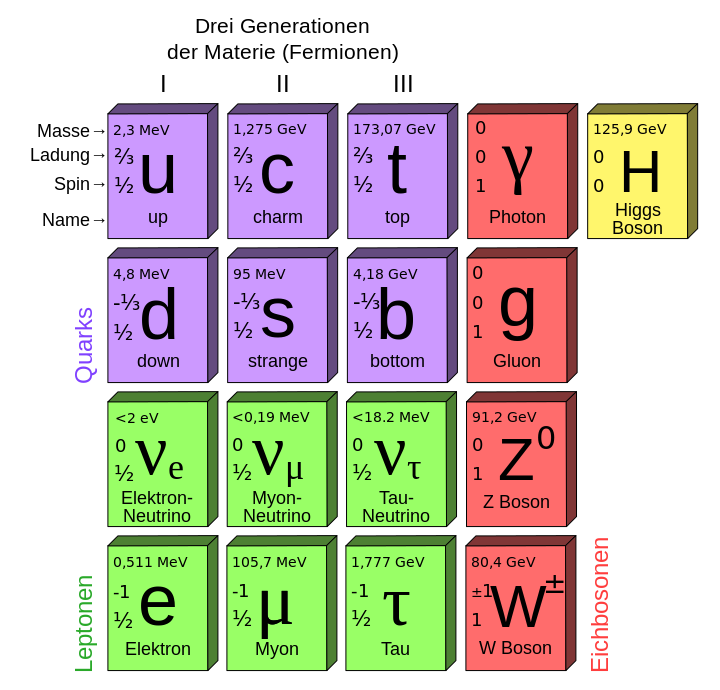
\includegraphics[width=\textwidth]{graphics/Standard_Model.png}
   \parbox[b]{12cm}{
     \caption[Standardmodell der Teilchenphysik]
             {\label{fig:Standardmodell} \it Die 12 fundamentalen Fermionen und 5 fundamentalen Bosonen des Standardmodells der Teilchenphysik,\\ Quelle: \cite{wiki:Standardmodell}}
   }
 \end{center}
\end{figure}

Insgesamt stimmen die experimentellen Ergebnisse gut mit den Vorhersagen des Standardmodells \"uberein. Dennoch reicht das Modell nicht aus, um s\"amtliche Ph\"anomene zu erkl\"aren. Im Modell werden beispielsweise masselose Neutrinos gefordert, allerdings ist durch die Beobachtung von Neutrinooszillationen erwiesen, dass massive Neutrinos existieren.

%% ===========================
\section{Assoziierte Higgs-Boson-Top-Quark-Paar-Produktion (\ttH)}
\label{ch:Theorie:sec:ttH}
%% ===========================

Da die Kopplungskonstante des Higgs-Mechanismus im Standardmodell von der Fermionenmasse abh\"angt, ist eine Untersuchung der Kopplung zwischen Top-Quark und Higgs-Boson aufgrund der hohen Masse des Top-Quarks verglichen mit anderen Quarkmassen, besonders interessant. Diese Kopplung kann w\"ahrend der assoziierten Produktion eines Higgs-Bosons mit einem Paar aus Top-Quark und Anti-Top-Quark untersucht werden. In Tabelle \ref{tab:quarkmasse} sind zum Vergleich die Quarkmassen aufgelistet.

\begin{table}[hhh]\parbox{12cm}{
  \caption[Quarkmassen]{\it Tabelle mit Quarkmassen, zusammengefasst aus{\rm \cite{Agashe:2014kda}}
  }\label{tab:quarkmasse}}
  \begin{center}
  \begin{tabular}{lll}
  \hline
  {\bf Quark} & {\bf Symbol} & {\bf Masse}  \\
  \hline \hline
     Up		& u & $2,3^{+0,7}_{-0,5}$~MeV \\
     Down	& d & $4,8^{+0,5}_{-0,3}$~MeV \\
     Strange& s & $95\pm 5$~MeV \\
     Charm	& c & $1,275\pm 0,025$~GeV \\ 
  	 Bottom & b & $4,18\pm 0,03$~GeV \\
     Top    & t & $ 173,07\pm 0,52\pm 0,72$~GeV \\                                   
  \hline
  \end{tabular}
  \end{center}
\end{table}

%% ===========================
\section{statistische Methoden}
\label{ch:Theorie:sec:statistischeMethoden}
%% ===========================


%% ===========================
\subsection{Receiver Operating Characteristic}
\label{ch:Algorithmen:subsec:ROC}
%% ===========================


%% ===========================
\subsection{Kolmogorov-Smirnov Test}
\label{ch:Algorithmen:subsec:KSTest}
%% ===========================